\documentclass{standalone}
\usepackage{tikz}
\usepackage{xcolor}
\usetikzlibrary{patterns, positioning}
\usetikzlibrary{shapes.misc}
\usepackage[outline]{contour}
\contourlength{1.5pt} 


\begin{document}
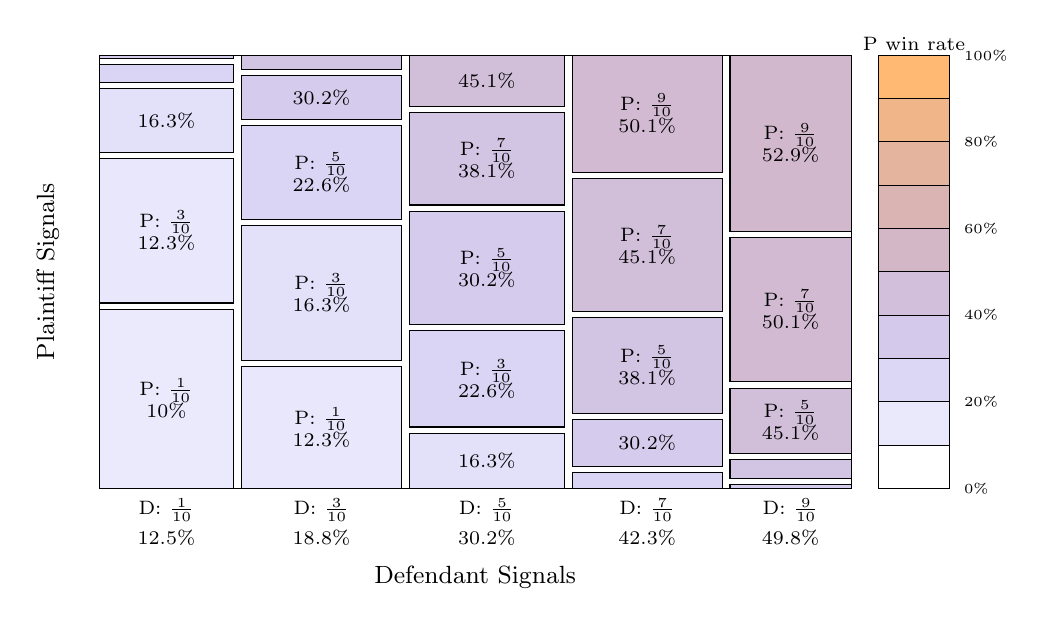
\begin{tikzpicture}
\newcommand{\DFractionOffset}{0.4}
\newcommand{\AxisLabelYAdjust}{-0.235}
\draw[draw=black] (0.6,2) rectangle (10.15,7.5);
\draw[fill=blue!90!orange!10!white!85!white, draw=black] (0.6,2) rectangle (2.3094,4.275);
\draw (1.454707986003248, 3.1374885320587182) node[font=\scriptsize, text=black, align=center] {P: $\frac{1}{10}$\\ 10\%};
\draw[fill=blue!88!orange!12!white!84!white, draw=black] (0.6,4.355) rectangle (2.3094,6.1893);
\draw (1.454707986003248, 5.272128857735475) node[font=\scriptsize, text=black, align=center] {P: $\frac{3}{10}$\\ 12.3\%};
\draw[fill=blue!84!orange!16!white!83!white, draw=black] (0.6,6.2693) rectangle (2.3094,7.0767);
\draw (1.454707986003248, 6.672972930358685) node[font=\scriptsize, text=black, align=center] {16.3\%};
\draw[fill=blue!77!orange!23!white!81!white, draw=black] (0.6,7.1567) rectangle (2.3094,7.3787);
\draw[fill=blue!70!orange!30!white!78!white, draw=black] (0.6,7.4587) rectangle (2.3094,7.5);
\draw (1.454707986003248, 1.6) node[anchor=north, font=\scriptsize, text=black] {12.5\%};
\draw (1.454707986003248, {1.6 + \DFractionOffset}) node[anchor=north, font=\scriptsize, text=black] {D: $\frac{1}{10}$};
\draw[fill=blue!88!orange!12!white!84!white, draw=black] (2.4094,2) rectangle (4.4373,3.5463);
\draw (3.4233487271283947, 2.773125198315836) node[font=\scriptsize, text=black, align=center] {P: $\frac{1}{10}$\\ 12.3\%};
\draw[fill=blue!84!orange!16!white!83!white, draw=black] (2.4094,3.6263) rectangle (4.4373,5.3375);
\draw (3.4233487271283947, 4.481874019355493) node[font=\scriptsize, text=black, align=center] {P: $\frac{3}{10}$\\ 16.3\%};
\draw[fill=blue!77!orange!23!white!81!white, draw=black] (2.4094,5.4175) rectangle (4.4373,6.6034);
\draw (3.4233487271283947, 6.010454174422164) node[font=\scriptsize, text=black, align=center] {P: $\frac{5}{10}$\\ 22.6\%};
\draw[fill=blue!70!orange!30!white!78!white, draw=black] (2.4094,6.6834) rectangle (4.4373,7.2401);
\draw (3.4233487271283947, 6.961739315215305) node[font=\scriptsize, text=black, align=center] {30.2\%};
\draw[fill=blue!62!orange!38!white!75!white, draw=black] (2.4094,7.3201) rectangle (4.4373,7.5);
\draw (3.4233487271283947, 1.6) node[anchor=north, font=\scriptsize, text=black] {18.8\%};
\draw (3.4233487271283947, {1.6 + \DFractionOffset}) node[anchor=north, font=\scriptsize, text=black] {D: $\frac{3}{10}$};
\draw[fill=blue!84!orange!16!white!83!white, draw=black] (4.5373,2) rectangle (6.509,2.7);
\draw (5.5231553572173, 2.3499829172013693) node[font=\scriptsize, text=black, align=center] {16.3\%};
\draw[fill=blue!77!orange!23!white!81!white, draw=black] (4.5373,2.78) rectangle (6.509,3.9996);
\draw (5.5231553572173, 3.389798456781574) node[font=\scriptsize, text=black, align=center] {P: $\frac{3}{10}$\\ 22.6\%};
\draw[fill=blue!70!orange!30!white!78!white, draw=black] (4.5373,4.0796) rectangle (6.509,5.5194);
\draw (5.5231553572173, 4.799533578249025) node[font=\scriptsize, text=black, align=center] {P: $\frac{5}{10}$\\ 30.2\%};
\draw[fill=blue!62!orange!38!white!75!white, draw=black] (4.5373,5.5994) rectangle (6.509,6.7717);
\draw (5.5231553572173, 6.185565352345248) node[font=\scriptsize, text=black, align=center] {P: $\frac{7}{10}$\\ 38.1\%};
\draw[fill=blue!55!orange!45!white!73!white, draw=black] (4.5373,6.8517) rectangle (6.509,7.5);
\draw (5.5231553572173, 7.175847313676428) node[font=\scriptsize, text=black, align=center] {45.1\%};
\draw (5.5231553572173, 1.6) node[anchor=north, font=\scriptsize, text=black] {30.2\%};
\draw (5.5231553572173, {1.6 + \DFractionOffset}) node[anchor=north, font=\scriptsize, text=black] {D: $\frac{5}{10}$};
\draw[fill=blue!77!orange!23!white!81!white, draw=black] (6.609,2) rectangle (8.5115,2.1995);
\draw[fill=blue!70!orange!30!white!78!white, draw=black] (6.609,2.2795) rectangle (8.5115,2.8729);
\draw (7.56028596229283, 2.576203012058096) node[font=\scriptsize, text=black, align=center] {30.2\%};
\draw[fill=blue!62!orange!38!white!75!white, draw=black] (6.609,2.9529) rectangle (8.5115,4.1678);
\draw (7.56028596229283, 3.5603291066829215) node[font=\scriptsize, text=black, align=center] {P: $\frac{5}{10}$\\ 38.1\%};
\draw[fill=blue!55!orange!45!white!73!white, draw=black] (6.609,4.2478) rectangle (8.5115,5.9372);
\draw (7.56028596229283, 5.092472724183342) node[font=\scriptsize, text=black, align=center] {P: $\frac{7}{10}$\\ 45.1\%};
\draw[fill=blue!50!orange!50!white!71!white, draw=black] (6.609,6.0172) rectangle (8.5115,7.5);
\draw (7.56028596229283, 6.758578630070364) node[font=\scriptsize, text=black, align=center] {P: $\frac{9}{10}$\\ 50.1\%};
\draw (7.56028596229283, 1.6) node[anchor=north, font=\scriptsize, text=black] {42.3\%};
\draw (7.56028596229283, {1.6 + \DFractionOffset}) node[anchor=north, font=\scriptsize, text=black] {D: $\frac{7}{10}$};
\draw[fill=blue!70!orange!30!white!78!white, draw=black] (8.6115,2) rectangle (10.15,2.0458);
\draw[fill=blue!62!orange!38!white!75!white, draw=black] (8.6115,2.1258) rectangle (10.15,2.363);
\draw[fill=blue!55!orange!45!white!73!white, draw=black] (8.6115,2.443) rectangle (10.15,3.2739);
\draw (9.380771346200675, 2.858462121515777) node[font=\scriptsize, text=black, align=center] {P: $\frac{5}{10}$\\ 45.1\%};
\draw[fill=blue!50!orange!50!white!71!white, draw=black] (8.6115,3.3539) rectangle (10.15,5.1876);
\draw (9.380771346200675, 4.2707782382864306) node[font=\scriptsize, text=black, align=center] {P: $\frac{7}{10}$\\ 50.1\%};
\draw[fill=blue!47!orange!53!white!71!white, draw=black] (8.6115,5.2676) rectangle (10.15,7.5);
\draw (9.380771346200675, 6.3838237240609885) node[font=\scriptsize, text=black, align=center] {P: $\frac{9}{10}$\\ 52.9\%};
\draw (9.380771346200675, 1.6) node[anchor=north, font=\scriptsize, text=black] {49.8\%};
\draw (9.380771346200675, {1.6 + \DFractionOffset}) node[anchor=north, font=\scriptsize, text=black] {D: $\frac{9}{10}$};
\node[font=\small, text=black] at (5.375, {1.1 + \AxisLabelYAdjust}) {Defendant Signals};
\node[font=\small, text=black, rotate=90] at (-0.050000000000000044, 4.75) {Plaintiff Signals};
\draw[draw=black] (10.5,2) rectangle (11.4,7.5);
\draw (10.95, 7.65) node[font=\scriptsize, text=black] {P win rate};
\draw[fill=blue!100!orange!0!white!88!white, draw=black] (10.5,2) rectangle (11.4,2.55);
\draw[fill=blue!89!orange!11!white!84!white, draw=black] (10.5,2.55) rectangle (11.4,3.1);
\draw[fill=blue!78!orange!22!white!81!white, draw=black] (10.5,3.1) rectangle (11.4,3.65);
\draw[fill=blue!67!orange!33!white!77!white, draw=black] (10.5,3.65) rectangle (11.4,4.2);
\draw[fill=blue!56!orange!44!white!73!white, draw=black] (10.5,4.2) rectangle (11.4,4.75);
\draw[fill=blue!44!orange!56!white!70!white, draw=black] (10.5,4.75) rectangle (11.4,5.3);
\draw[fill=blue!33!orange!67!white!66!white, draw=black] (10.5,5.3) rectangle (11.4,5.85);
\draw[fill=blue!22!orange!78!white!62!white, draw=black] (10.5,5.85) rectangle (11.4,6.4);
\draw[fill=blue!11!orange!89!white!59!white, draw=black] (10.5,6.4) rectangle (11.4,6.95);
\draw[fill=blue!0!orange!100!white!55!white, draw=black] (10.5,6.95) rectangle (11.4,7.5);
\draw (11.46, 2) node[anchor=west, font=\tiny, text=black] {0\%};
\draw (11.46, 3.1) node[anchor=west, font=\tiny, text=black] {20\%};
\draw (11.46, 4.2) node[anchor=west, font=\tiny, text=black] {40\%};
\draw (11.46, 5.3) node[anchor=west, font=\tiny, text=black] {60\%};
\draw (11.46, 6.4) node[anchor=west, font=\tiny, text=black] {80\%};
\draw (11.46, 7.5) node[anchor=west, font=\tiny, text=black] {100\%};


\end{tikzpicture}
\end{document}